\chapter{Estado del arte}


\section{¿Qué es una ECU?}


Una ECU \textit{Electronic Control Unit} es un sistema empotrado, que consta de un microcontrolador especializado en la automoción. [1] (embitel.com) Permite, junto con el software y los protocolos de comunicación, y el conjunto de sensores y actuadores, controlar los sistemas eléctricos y subsistemas en un vehículo para su correcto funcionamiento. 
Esencialmente se encarga de recibir la información que le aportan los sensores acerca del entorno, procesar esa información para completar diversas tareas y, en muchos casos, enviar las directrices que se requieren a los actuadores de los componentes.\newline

\begin{figure}[h]
    \centering
    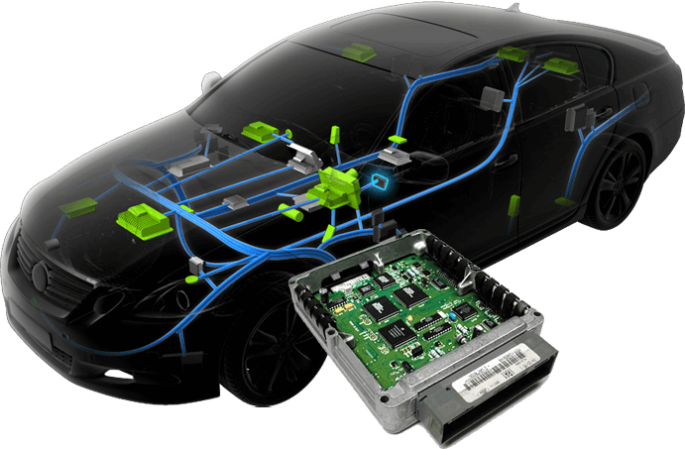
\includegraphics[width=0.5\textwidth]{imagenes/ECU_autotechdrive.png}
    \caption{Imagen de una ECU y su impacto en un vehículo. Extraído de: []}
\end{figure}

\subsection{Evolución e historia de la gestión de datos los vehículos}

Las siglas ECU no siempre han tenido el mismo significado. Inicialmente, cuando se comenzaron a utilizar (en torno a los años setenta), era para hablar de la unidad de control del motor \textit{\textbf{Engine Control Unit}}. Podemos desgajar los grandes cambios en lo siguiente[4]:

\begin{itemize}

    \item \textbf{Años 70} - Inicialmente eran dispositivos extremadamente simples, que solamente controlaban un par de solenoides en el \textbf{carburador}, el encargado de preparar la mezcla de aire y combustible en motores de gasolina, de manera que el vehículo pudiera obtener la máxima potencia de salida de la manera más eficiente.

    \begin{figure}[h]
        \centering
        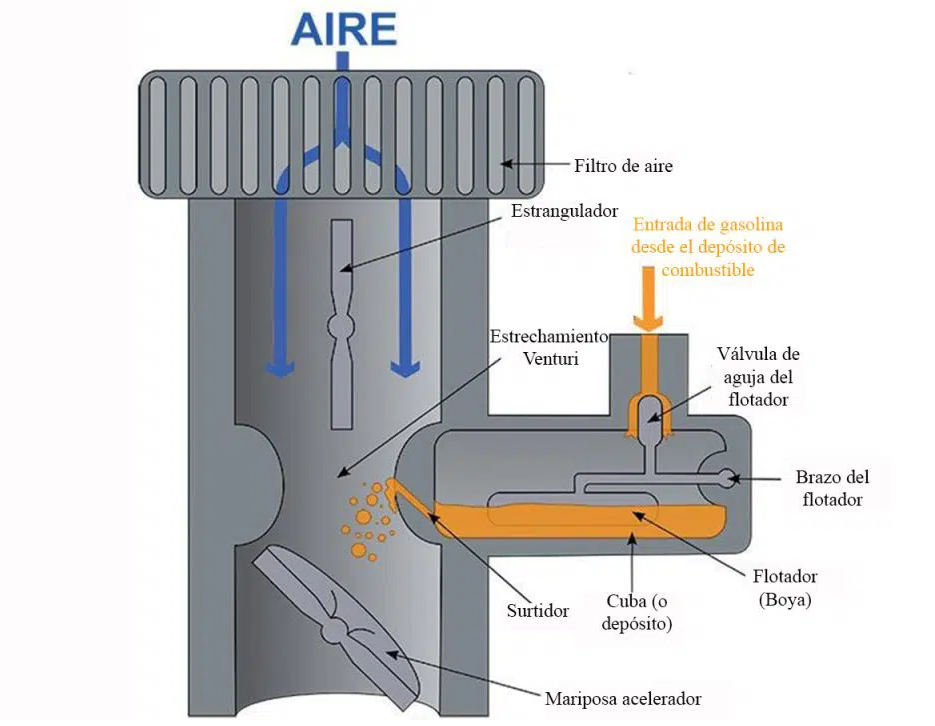
\includegraphics[width=0.5\textwidth]{imagenes/esquema_carburador.png}
        \caption{Imagen simplificada de un carburador sus partes. Extraído de: [5]}
    \end{figure}
 
    \item \textbf{Años 80} - En esta época se comenzaron a utilizar los \textbf{reguladores de presión de combustible}, un componente que busca controlar y mantener constante la presión del combustible. Permitió a los fabricantes de vehículos tener mayor control a la hora de no dañar otros componentes, tales como inyectores o los conductos del sistema en general [5]. En este punto, la unidad de control del motor ya era la principal responsable de los sistemas de combustión. También comenzaron a utilizar el \textbf{Control de Lambda} para modificar parámetros de la misma, y alcanzar una mayor eficiencia.

    \begin{figure}[h]
        \centering
        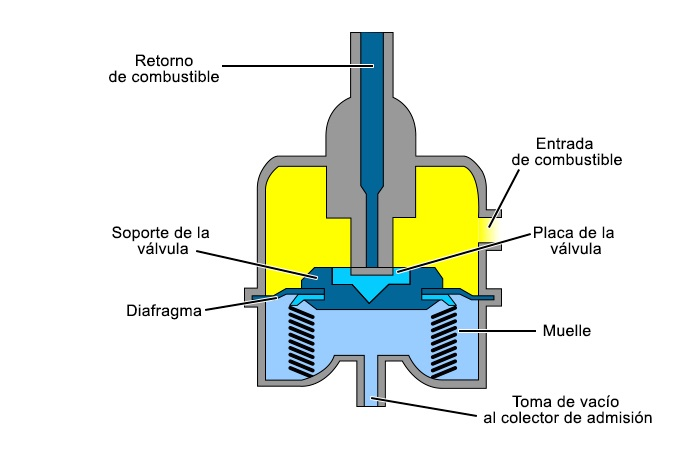
\includegraphics[width=0.6\textwidth]{imagenes/esquema_rpc.png}
        \caption{Imagen simplificada de un regulador de combustible y sus partes. Extraído de: [7]}
    \end{figure}


    \item \textbf{Años 90} - Las ECUs añadieron un conjunto de medidas para mejorar la seguridad en el vehículo, siendo el \textbf{ABS ó Antiblockiersystem} la más relevante. Esta tecnología, aún en uso en los vehículos actuales, se encarga de variar la fuerza de frenado al detectar mediante sensores de revoluciones en las ruedas, evitando así que estas se bloqueen y perdamos el control del vehículo. El uso de las ECUs se extiende hacia los motores diésel, teniendo un papel esencial en el desarrollo de los vehículos turbodiésel.

    \begin{figure}[h]
        \centering
        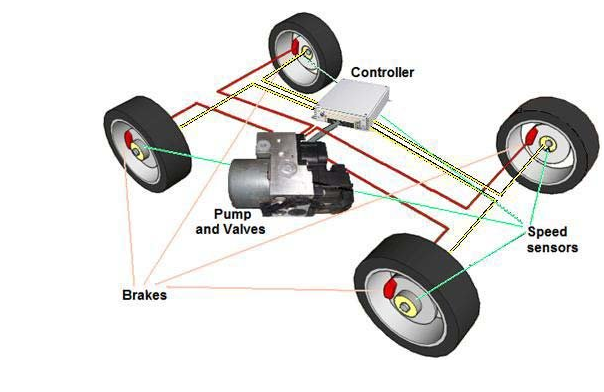
\includegraphics[width=0.5\textwidth]{imagenes/esquema_abs.png}
        \caption{Imagen simplificada del ABS y sus partes. Extraído de: [8]}
    \end{figure}
    
 
    \item \textbf{Años 2000} - Las unidades de control comienzan a incluir la tecnología \textit{\textbf{drive-by-wire}}, un formalismo para definir la sustitución de controles mecánicos tradicionales por sistemas electrónicos [9], así como también se añade control del turbo y sistemas para minimizar emisiones y cumplir con los protocolos pertinentes.
       

    \begin{figure}[h]
        \centering
        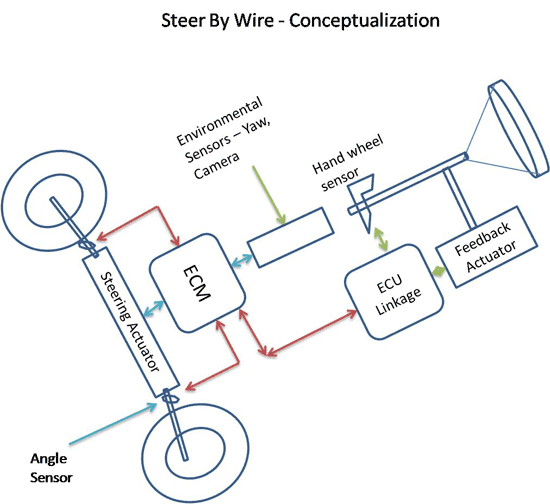
\includegraphics[width=0.5\textwidth]{imagenes/esquema_dbw.png}
        \caption{Conceptualización del sistema \textit{drive-by-wire}. Extraído de: [10]}
    \end{figure}
          

    \item \textbf{Años 2010-Actualidad} - La centralita del motor controla todo el sistema de mezcla del combustible, emisiones, refrigeración y sistemas de aceleración del vehículo. Dejan de ser dispositivos simples, ahora tienen cientos de entradas, decenas de sensores, y forman parte de un conjunto de ECUs (ya utilizando la acepción actual del término: \textit{Electronic Control Unit}), cada una focalizada en un conjunto de tareas, yendo desde el propio control del motor, hasta los sistemas de infoentretenimiento del vehículo. 
       

    \begin{figure}[h]
        \centering
        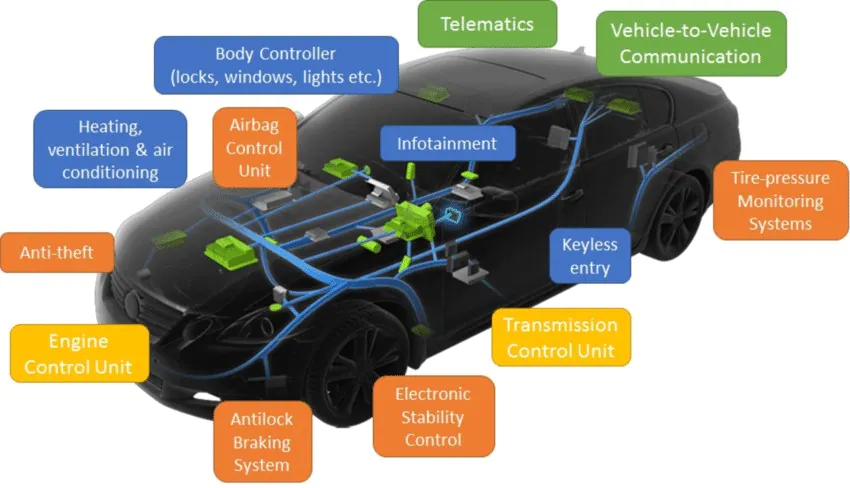
\includegraphics[width=0.5\textwidth]{imagenes/ECU_autotechdrive_completa.png}
        \caption{Representación de las distintas ECUs que controlan un vehículo. Extraído de: [11]}
    \end{figure}
              
\end{itemize}



\subsection{La ECU en los vehículos: El mejor amigo del conductor}

El ser humano ha hecho grandes avances en la tecnología, y esto no podría ser menos en los vehículos. Las ECU que, como se ha visto en el apartado anteror, inicialmente no tenían tanta importancia, ahora se han convertido en algo fundamental para nosotros. Estas centralitas, que antiguamente servían únicamente para gestionar la inyección de combustible en el el motor, ahora tienen multitud de utilidades para cada una de las partes del vehículo.

Gracias a estos sistemas, podemos obtener desde una mayor eficiencia en el uso de la fuente de energía (ya sea combustible fósil o electricidad), un control más específico de los mapas motor para mayor potencia, recolección de datos relevantes del vehículo, e incluso algunas mejoras \textit{Quality of Life (QoL)} que nos permitan una conducción más cómoda. 

Muchos de estos sistemas no solamente inciden en la eficiencia y comodidad, sino también en la seguridad del conductor y de los pasajeros abordo. Algunas de las medidas más relevantes, que vamos a categorizar entre activas y pasivas, son las siguientes[11]:

\begin{enumerate}
    \item \textbf{Seguridad activa} - Conjunto de medidas que proporcionan mayor estabilidad al vehículo, buscando evitar el accidente a priori.
    \begin{itemize}
        \item Luces adaptativas: Esta tecnología se basa en el uso de una matriz de LEDs en las luces delanteras, al contrario de la tradicional bombilla incandescente usada anteriormente. Los beneficios de este diseño son múltiples, pues permite modificar el haz de luz para evitar posibles deslumbramientos a otros usuarios de la vía, así como también adaptarse a las condiciones de la carretera, e iluminar más eficazmente el trazado.

        \begin{figure}[h]
            \centering
            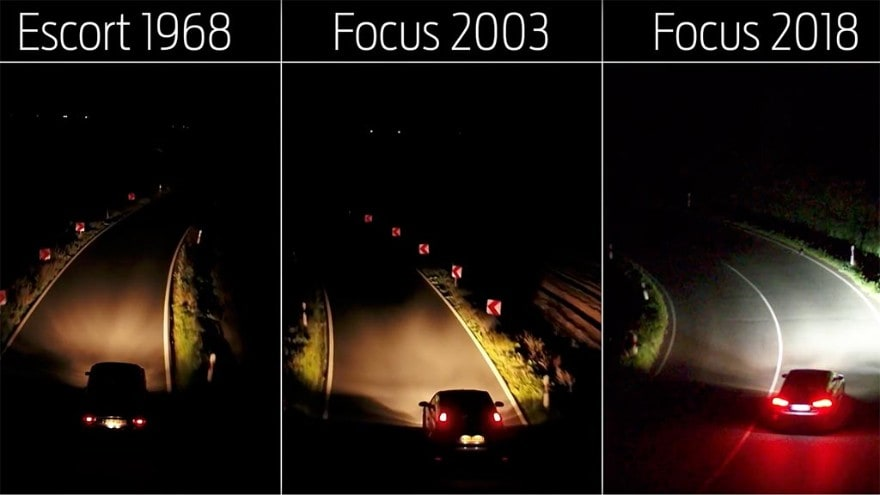
\includegraphics[width=0.7\textwidth]{imagenes/adaptive_lights.png}
            \caption{Comparación de la iluminación en los vehículos tras los años. Extraído de: [13]}
        \end{figure}
     


    \end{itemize}

    \item \textbf{Seguridad pasiva} - Conjunto de medidas que actúan una vez ha sucedido el accidente o el mal funcionamiento. Tienen el objetivo de minimizar los daños.
\end{enumerate}




\section{Fundamentos de una ECU}
\subsection{La introducción de sensores y actuadores}
*Meter un grafico del funcionamiento de un sistema con sens. y act.
\subsection{Ventajas e inconvenientes} 
\section{El OBD y su utilidad}
\section{Código Abierto, Software Libre y Licencias}

El software libre y sus licencias \cite{gplv3} ha permitido llevar a cabo una expansión del
aprendizaje de la informática sin precedentes.